\chapter{Flux de Càrregues}
\index{flux de càrregues}\label{chap:flux_carregues}

\section{Introducció}

Es tracta en aquest capítol el mètode de resolució del problema del flux de càrregues en
sistemes elèctrics de potència.

Quan les dades que es coneixen de les càrregues d'una xarxa no són
les seves impedàncies o admitàncies sinó les potències que
absorbeixen, no podem emprar el mètode dels nusos descrit en el
capítol \ref{chap:nusos} per tal de resoldre-la.

En aquest cas, el mètode de resolució es basa en escriure per a cada
nus les equacions pertinents del balanç de potència activa i
reactiva, i resoldre-les. La solució del sistema d'equacions
resultant ens proporcionarà les tensions de tots els nusos de la
xarxa i el flux de potència activa i reactiva entre els seus nusos.

El sistema d'equacions que cal resoldre és no lineal, i per tant
cal emprar algun mètode numèric per obtenir-ne la solució, com ara el
de Newton-Raphson. \index{Newton-Raphson} Aquí, no obstant, no
s'explicarà cap mètode numèric de resolució de sistemes d'equacions
no lineals, ja que això cau fora de l'abast d'aquest llibre; això
però, no hauria de suposar cap problema, ja que actualment aquests
sistemes d'equacions es poden resoldre fàcilment amb programes
d'ordinador de càlcul matemàtic com ara els programes
\emph{Mathematica®} o \emph{MATLAB®}, o amb calculadores
científiques com ara les \emph{Hewlett-Packard}.
\index{Mathematica@\emph{Mathematica®}}
\index{MATLAB@\emph{MATLAB®}}

\section{Models matemàtics} \index{flux de càrregues!models matemàtics}

En els estudis de flux de càrregues els elements que es consideren són:
\begin{itemize}
   \item Càrregues
   \item Línies elèctriques
   \item Transformadors amb regulació variable (amb desfasament o sense)
\end{itemize}

\subsection{Càrregues}

Les càrregues venen sempre definides per la potència que absorbeixen, és a dir, es consideren fonts de potència constant.

\subsection{Línies elèctriques} \index{linies@línies elèctriques}

Les línies elèctriques es modelen mitjançant un circuit equivalent
per fase en «$\piup$», format per una impedància longitudinal i dues
admitàncies transversals, tal com es pot veure en la Figura
\vref{pic:equiv_linia}. En aquesta figura s'ha suposat que la línia
està connectada entre els nusos 1 i 2; les admitàncies transversals
tenen sempre un extrem connectat a terra (nus 0 de referència).
\index{linies@línies elèctriques!circuit equivalent en
\guillemotleft$\piup$\guillemotright}

\begin{center}
    \input{Imatges/Cap-FluxCarregues-Linia.pdf_tex}
    \captionof{figure}{Circuit equivalent d'una línia elèctrica}
    \label{pic:equiv_linia}
\end{center}

A partir dels paràmetres propis d'una línia, la seva impedància
longitudinal  total per fase $\cmplx{Z}\ped{t}$ i la seva admitància
transversal total per fase $\cmplx{Y}\ped{t}$, definim la impedància
característica $\cmplx{Z}\ped{c}$ i l'angle característic
$\cmplx{\theta}\ped{c}$ de la línia: \index{linies@línies
elèctriques!impedància característica} \index{linies@línies
elèctriques!angle característic} \index{Zc@$\cmplx{Z}\ped{c}$}
\index{$\cmplx{\theta}\ped{c}$}
\begin{equation}
   \cmplx{Z}\ped{c} = \sqrt{\frac{\cmplx{Z}\ped{t}}{\cmplx{Y}\ped{t}}} \qquad \qquad
   \cmplx{\theta}\ped{c} = \sqrt{\cmplx{Z}\ped{t} \,\cmplx{Y}\ped{t} }
\end{equation}

Amb aquests dos paràmetres, les equacions hiperbòliques de
transmissió d'una línia són: \index{linies@línies
elèctriques!equacions hiperbòliques de transmissió}
\begin{equation}\label{eq:linia_eq_trans}
   \cmplx{U}_1 = \cmplx{U}_2 \cosh \cmplx{\theta}\ped{c}  + \cmplx{I}_2 \,\cmplx{Z}\ped{c} \sinh \cmplx{\theta}\ped{c}   \qquad \qquad
   \cmplx{I}_1 = \cmplx{U}_2 \, \frac{\sinh \cmplx{\theta}\ped{c}}{\cmplx{Z}\ped{c}}  +   \cmplx{I}_2 \cosh \cmplx{\theta}\ped{c}
\end{equation}

D'altra banda, en el circuit de la Figura \vref{pic:equiv_linia} es compleix:
\begin{equation}\label{eq:linia_eq}
   \cmplx{I}_2 = \frac{\cmplx{U}_1 - \cmplx{U}_2}{\cmplx{Z}_\piup} - \cmplx{Y}_\piup\, \cmplx{U}_2
   \quad \rightarrow\quad
   \cmplx{U}_1 = (1 + \cmplx{Z}_\piup\,\cmplx{Y}_\piup ) \cmplx{U}_2 + \cmplx{Z}_\piup\,\cmplx{I}_2
\end{equation}

Identificant entre si els termes de les equacions
\eqref{eq:linia_eq_trans} i \eqref{eq:linia_eq}, obtenim els
paràmetres del circuit equivalent de la línia.
\begin{alignat}{2}
   \cmplx{Z}_\piup &= \cmplx{Z}\ped{c} \sinh \cmplx{\theta}\ped{c} &&= \cmplx{Z}\ped{t} \,
   \frac{\sinh \cmplx{\theta}\ped{c}}{\cmplx{\theta}\ped{c}} \\[1.5ex]
   \cmplx{Y}_\piup &= \frac{\tanh (\cmplx{\theta}\ped{c} / 2) }{\cmplx{Z}\ped{c}} &&=
   \frac{\cmplx{Y}\ped{t}}{2} \, \frac{\tanh (\cmplx{\theta}\ped{c} / 2)}{\cmplx{\theta}\ped{c} / 2}
\end{alignat}

Ara bé, en la majoria dels casos es compleix: $|\cmplx{\theta}\ped{c}| \ll 1$, i utilitzant els desenvolupaments en sèrie de Taylor de les funcions $\sinh$ i $\tanh$, al voltant de 0, tenim:
\begin{align}
   \cmplx{Z}_\piup &= \cmplx{Z}\ped{t} \, \left[ 1 + \frac{\cmplx{\theta}\ped{c}^2}{3!} +
   \frac{\cmplx{\theta}\ped{c}^4}{5!} + \cdots \right] \approx \cmplx{Z}\ped{t} \\[1.5ex]
   \cmplx{Y}_\piup &= \frac{\cmplx{Y}\ped{t}}{2} \,\left[ 1 - \frac{(\cmplx{\theta}\ped{c}/2)^2}{3} + \frac{2 (\cmplx{\theta}\ped{c}/2)^4}{15} - \cdots \right] \approx \frac{\cmplx{Y}\ped{t}}{2}
\end{align}

Utilitzant aquests valors, la contribució d'una línia elèctrica a
la matriu d'admitàncies de nus $\mcmplx{Y}\ped{N}$ de la xarxa a la
qual pertany, és: \index{linies@línies elèctriques!matriu
d'admitàncies de nus $\mcmplx{Y}\ped{N}$}
\index{matriu!d'admitàncies de nus $\mcmplx{Y}\ped{N}$}
\begin{equation}
   \mcmplx{Y}\ped{N} = \begin{pmatrix}
     \dfrac{\cmplx{Y}\ped{t}}{2} + \dfrac{1}{\cmplx{Z}\ped{t}} & -\dfrac{1}{\cmplx{Z}\ped{t}}\\[2.5ex]
     -\dfrac{1}{\cmplx{Z}\ped{t}} & \dfrac{\cmplx{Y}\ped{t}}{2} + \dfrac{1}{\cmplx{Z}\ped{t}}
   \end{pmatrix}
\end{equation}

Els fluxos de potència a través de la línia, $\cmplx{S}_{12}$ (del
nus 1 al 2), i $\cmplx{S}_{21}$ (del nus 2 a l'1), venen donats per
les expressions:\index{linies@línies elèctriques!fluxos de potència}
\begin{align}
   \cmplx{S}_{12} &= \cmplx{U}_1 \left[ \left( \frac{\cmplx{Y}\ped{t}}{2} + \frac{1}{\cmplx{Z}\ped{t}} \right) \cmplx{U}_1 - \frac{1}{\cmplx{Z}\ped{t}} \cmplx{U}_2 \right]^{\,*} = \cmplx{U}_1 \left[ \frac{\cmplx{Y}\ped{t}}{2}\, \cmplx{U}_1 + \frac{\cmplx{U}_1 - \cmplx{U}_2}{\cmplx{Z}\ped{t}} \right]^{\,*} \label{eq:lin_s12}
   \\[1.5ex]
   \cmplx{S}_{21} &= \cmplx{U}_2 \left[ \left( \frac{\cmplx{Y}\ped{t}}{2} + \frac{1}{\cmplx{Z}\ped{t}} \right) \cmplx{U}_2 - \frac{1}{\cmplx{Z}\ped{t}} \cmplx{U}_1 \right]^{\,*} = \cmplx{U}_2 \left[ \frac{\cmplx{Y}\ped{t}}{2} \,\cmplx{U}_2 + \frac{\cmplx{U}_2 - \cmplx{U}_1}{\cmplx{Z}\ped{t}} \right]^{\,*} \label{eq:lin_s21}
\end{align}

Finalment, les pèrdues de transmissió $\Delta\cmplx{S}$ en la  línia venen donades per
l'expressió:\index{linies@línies elèctriques!pèrdues de transmissió}
\begin{equation}
   \Delta\cmplx{S} = \cmplx{S}_{12} + \cmplx{S}_{21} = \left[ \frac{\cmplx{Y}\ped{t}}{2} + \frac{1}{\cmplx{Z}\ped{t}} \right]^{\,*} \Big[ |\cmplx{U}_1|^2 + |\cmplx{U}_2|^2 \Big] - 2 \, \frac{\Re (\cmplx{U}_1^* \cmplx{U}_2)}{\cmplx{Z}\ped{t}^*}
\end{equation}

\subsection{Transformadors amb regulació variable i desfasament}
\index{transformadors amb regulació variable i desfasament}

Els transformadors amb regulació variable i desfasament es modelen
mitjançant un transformador ideal en sèrie amb una impedància
(vegeu també la secció \ref{sec:connex-index-horari}), tal
com es pot veure en la Figura \vref{pic:equiv_trafo_reg_decal}. En
aquesta figura s'ha suposat que el transformador està connectat
entre els nusos 1 i 2; el punt de referència del transformador és
sempre  el terra (nus 0 de referència). \index{transformadors amb
regulació variable i desfasament!circuit equivalent}

\begin{center}
    \input{Imatges/Cap-FluxCarregues-Trafo.pdf_tex}
    \captionsetup{justification=raggedright,margin={3.5cm,3.5cm},oneside}
    \captionof{figure}{Circuit equivalent d'un transformador amb regulació variable i desfasament}
    \label{pic:equiv_trafo_reg_decal}
\end{center}

En l'esquema anterior, $\cmplx{Z}\ped{cc}$ és la impedància de curtcircuit per fase del transformador, i $\cmplx{m}\!:\!1$ n'és la
relació de transformació. El paràmetre $\cmplx{m}$ és un valor
complex ja que el transformador a més de variar el mòdul de la
tensió, també en varia  l'argument; les tensions primària i
secundària tenen, per tant,  diferent mòdul i un desfasament entre els
seus arguments.

Si la impedància es volgués representar en el primari del
transformador, el seu valor seria $|\cmplx{m}|^2 \cmplx{Z}\ped{cc}$.

En el circuit de la Figura \vref{pic:equiv_trafo_reg_decal} es
compleix: \index{transformadors amb regulació variable i
desfasament!equacions de funcionament}
\begin{equation}
   \cmplx{U}_1 = \cmplx{m} \,\cmplx{U} = \cmplx{m}\,
   [\cmplx{U}_2+\cmplx{Z}\ped{cc}\cmplx{I}_2]
   \qquad\qquad
   \cmplx{I}_1 = \frac{\cmplx{I}}{\cmplx{m}^*} = \frac{\cmplx{I}_2}{\cmplx{m}^*}
   \qquad\qquad
   \cmplx{U}_1 \cmplx{I}_1^* = \cmplx{U} \,\cmplx{I}^*
\end{equation}

Utilitzant aquestes tres equacions podem escriure:
\begin{equation}
   \cmplx{I}_1 = \frac{\cmplx{U}_1}{|\cmplx{m}|^2 \cmplx{Z}\ped{cc}} - \frac{\cmplx{U}_2}
   {\cmplx{m}^* \cmplx{Z}\ped{cc}} \qquad\qquad
   - \cmplx{I}_2 = - \frac{\cmplx{U}_1}{\cmplx{m} \,\cmplx{Z}\ped{cc}} + \frac{\cmplx{U}_2}
   {\cmplx{Z}\ped{cc}}
\end{equation}

Aquestes equacions ens permeten escriure directament la
contribució d'un transformador amb regulació variable i desfasament, a
la matriu d'admitàncies de nus $\mcmplx{Y}\ped{N}$ de la xarxa a la
qual pertany: \index{transformadors amb regulació variable i
desfasament!matriu d'admitàncies de nus $\mcmplx{Y}\ped{N}$}
\index{matriu!d'admitàncies de nus $\mcmplx{Y}\ped{N}$}
\begin{equation} \label{eq:yn_trafo_reg_decal}
   \mcmplx{Y}\ped{N} = \begin{pmatrix}
     \dfrac{1}{|\cmplx{m}|^2 \cmplx{Z}\ped{cc}} & - \dfrac{1}
   {\cmplx{m}^* \cmplx{Z}\ped{cc}} \\[2.5ex]
     - \dfrac{1}{\cmplx{m} \,\cmplx{Z}\ped{cc}} & \dfrac{1}
   {\cmplx{Z}\ped{cc}}
   \end{pmatrix}
\end{equation}

Com es pot veure, $\mcmplx{Y}\ped{N}(1,2) \neq
\mcmplx{Y}\ped{N}(2,1)$; això ens indica que no existeix un esquema
equivalent en «$\piup$» del transformador, format únicament per
elements passius.

Els fluxos de potència a través del transformador, $\cmplx{S}_{12}$
(del nus 1 al 2), i $\cmplx{S}_{21}$ (del nus 2 a l'1), venen donats
per les expressions: \index{transformadors amb regulació variable i
desfasament!fluxos de potència}
\begin{alignat}{2}
   \cmplx{S}_{12} &= \cmplx{U}_1 \left[ \frac{\cmplx{U}_1}{|\cmplx{m}|^2 \cmplx{Z}\ped{cc}} - \frac{\cmplx{U}_2}{\cmplx{m}^* \cmplx{Z}\ped{cc}} \right]^{\,*} &&= \frac{\cmplx{U}_1}{\cmplx{m}\, \cmplx{Z}\ped{cc}^*} \left[ \frac{\cmplx{U}_1}{\cmplx{m}} - \cmplx{U}_2 \right]^{\,*} \label{eq:s12_trafo_reg_decal} \\[1.5ex]
   \cmplx{S}_{21} &= \cmplx{U}_2 \left[ - \frac{\cmplx{U}_1}{\cmplx{m} \,\cmplx{Z}\ped{cc}} + \frac{\cmplx{U}_2} {\cmplx{Z}\ped{cc}} \right]^{\,*} &&= \frac{\cmplx{U}_2}{\cmplx{Z}\ped{cc}^*} \left[  \cmplx{U}_2 - \frac{\cmplx{U}_1}{\cmplx{m}}  \right]^{\,*} \label{eq:s21_trafo_reg_decal}
\end{alignat}

Finalment, les pèrdues de transmissió $\Delta\cmplx{S}$ del transformador venen donades per l'expressió:
\index{transformadors amb regulació variable i desfasament!pèrdues de
transmissió}
\begin{equation} \label{eq:ds_trafo_reg_decal}
   \Delta\cmplx{S} = \cmplx{S}_{12} + \cmplx{S}_{21} = \frac{1}{\cmplx{Z}\ped{cc}^*}  \left|
    \frac{\cmplx{U}_1}{\cmplx{m}} - \cmplx{U}_2 \right|^2
\end{equation}


\subsection{Transformadors amb regulació variable sense desfasament} \label{sec:trafo_reg}
\index{transformadors amb regulació variable sense desfasament}

Aquest és un cas particular de l'anterior, on el transformador no
origina desfasament entre les tensions primària i secundària.
En aquest cas, la relació de transformació $m\!:\!1$ és un valor real.

A partir de l'equació  \eqref{eq:yn_trafo_reg_decal}, substituint
$\cmplx{m}$ per $m$, obtenim la contribució d'un transformador amb
regulació variable sense desfasament, a la matriu d'admitàncies de nus
$\mcmplx{Y}\ped{N}$ de la xarxa a la qual pertany:
\index{transformadors amb regulació variable sense desfasament!matriu
d'admitàncies de nus $\mcmplx{Y}\ped{N}$}
\index{matriu!d'admitàncies de nus $\mcmplx{Y}\ped{N}$}
\begin{equation}
   \mcmplx{Y}\ped{N} = \begin{pmatrix}
     \dfrac{1}{m^2 \cmplx{Z}\ped{cc}} & - \dfrac{1}{m \,\cmplx{Z}\ped{cc}} \\[2.5ex]
     - \dfrac{1}{m \,\cmplx{Z}\ped{cc}} & \dfrac{1}{\cmplx{Z}\ped{cc}}
   \end{pmatrix}
\end{equation}

Anàlogament podem obtenir els fluxos de potència a través del
transformador, $\cmplx{S}_{12}$ (del nus 1 al 2), i $\cmplx{S}_{21}$
(del nus 2 a l'1), i les seves pèrdues de transmissió
$\Delta\cmplx{S}$, a partir de les equacions
\eqref{eq:s12_trafo_reg_decal},  \eqref{eq:s21_trafo_reg_decal} i
\eqref{eq:ds_trafo_reg_decal}: \index{transformadors amb regulació
variable sense desfasament!fluxos de potència} \index{transformadors
amb regulació variable sense desfasament!pèrdues de transmissió}
\begin{align}
   \cmplx{S}_{12} &= \cmplx{U}_1 \left[ \frac{\cmplx{U}_1}{m^2 \cmplx{Z}\ped{cc}} - \frac{\cmplx{U}_2}{m \cmplx{Z}\ped{cc}} \right]^{\,*} = \frac{\cmplx{U}_1}{m \,\cmplx{Z}\ped{cc}^*} \left[ \frac{\cmplx{U}_1}{m} - \cmplx{U}_2 \right]^{\,*}  \\[1.5ex]
   \cmplx{S}_{21} &= \cmplx{U}_2 \left[ - \frac{\cmplx{U}_1}{m \,\cmplx{Z}\ped{cc}} + \frac{\cmplx{U}_2} {\cmplx{Z}\ped{cc}} \right]^{\,*} = \frac{\cmplx{U}_2}{\cmplx{Z}\ped{cc}^*} \left[  \cmplx{U}_2 - \frac{\cmplx{U}_1}{m}  \right]^{\,*} \\[1.5ex]
 \Delta\cmplx{S} &= \cmplx{S}_{12} + \cmplx{S}_{21} = \frac{1}{\cmplx{Z}\ped{cc}^*}  \left|
    \frac{\cmplx{U}_1}{m} - \cmplx{U}_2 \right|^2
\end{align}


El circuit equivalent d'aquest tipus de transformador també és el de la
 Figura \vref{pic:equiv_trafo_reg_decal}, substituint $\cmplx{m}\!:\!1$ per $m\!:\!1$; no
 obstant, atès que en aquest cas es compleix $\mcmplx{Y}\ped{N}(1,2) = \mcmplx{Y}\ped{N}(2,1)$, també
 existeix un circuit equivalent en «$\piup$» format per una impedància longitudinal i dues admitàncies transversals, tal com es pot veure en la Figura  \vref{pic:equiv_trafo_reg}.
\index{transformadors amb regulació variable sense desfasament!circuit
equivalent en \guillemotleft$\piup$\guillemotright}

\begin{center}
    \input{Imatges/Cap-FluxCarregues-Trafo-Pi.pdf_tex}
    \captionsetup{justification=raggedright,margin={3.5cm,3.5cm},oneside}
    \captionof{figure}{Circuit equivalent d'un transformador amb regulació variable sense desfasament}
    \label{pic:equiv_trafo_reg}
\end{center}

Els valors dels paràmetres d'aquest circuit equivalent són:
\begin{align}
   \cmplx{Z}_\piup &= m \, \cmplx{Z}\ped{cc} \\[1.5ex]
   \cmplx{Y}_{\piup_1} &= \frac{1-m}{m^2 \,\cmplx{Z}\ped{cc}} \\[1.5ex]
   \cmplx{Y}_{\piup_2} &= \frac{m-1}{m\, \cmplx{Z}\ped{cc}}
\end{align}

\section{Tipus de nusos} \index{flux de càrregues!tipus de nusos}

Cadascun dels nusos d'un sistema elèctric de potència té quatre
magnituds associades: les potències activa i reactiva injectades des
de l'exterior de la xarxa, i el mòdul i l'argument de la seva
tensió.

Usualment, en cada nus del sistema es coneixen dues de les quatre
magnituds anteriors; segons quines siguin aquestes magnituds es
poden distingir els següents tipus de nusos:
\begin{itemize}
    \item \textbf{Nus de potencial zero}. El terra és sempre el nus de referència o de potencial zero de la
    xarxa, i per tant, totes les tensions de la xarxa hi són referides.
    Al terra se li assigna el número de nus 0, i per tant no forma part de la matriu d'admitàncies de nus de la xarxa.
\index{nus!de potencial zero}\index{nus!de referència}

   \item \textbf{Nus flotant}. És un nus on es manté constant la tensió en mòdul i argument,
   essent incògnites les potències activa i reactiva injectades a la xarxa des de l'exterior.
    Generalment, acostuma a ser el nus que més s'aproxima a un nus de potència infinita. Des del
    punt de vista de la xarxa, correspon clarament a un generador ideal de tensió.
    \index{nus!flotant}

Només hi pot haver un nus d'aquest tipus en tota la xarxa.
   \item \textbf{Nus de tensió controlada}. En aquest nus es coneix el mòdul de la tensió i la
   potència activa injectada a la xarxa des de l'exterior, essent incògnites l'argument de la tensió i la potència
   reactiva injectada des de l'exterior. En aquests nusos sovint s'imposen límits a la potència reactiva.
\index{nus!de tensió controlada}

   \item \textbf{Nus de càrrega}. En aquest nus es coneixen les potències activa i reactiva
   injectades a la xarxa des de l'exterior, essent incògnites el mòdul i l'argument de la tensió.
   Aquests nusos poden ser tant de consum com de generació.
   \index{nus!de càrrega}

En els nusos on incideix un transformador amb relació de
transformació variable sense desfasament, hi pot haver tres magnituds
conegudes: les potències activa i reactiva injectades i el mòdul de
la tensió, el qual es vol mantenir constant mitjançant l'ajust de la
relació de transformació; les incògnites són, per tant, l'argument de
la tensió i la citada relació de transformació del transformador.
\end{itemize}

En la Taula \vref{taula:tipus_nusos} es resumeix el que s'ha exposat
sobre els diferents tipus de nusos en un sistema elèctric de
potència.

\begin{center}
\begin{threeparttable}
   \caption{Tipus de nusos en un sistema elèctric de potència} \label{taula:tipus_nusos}
   \begin{tabular}{lccccc}
   \toprule[1pt]
   \multirow{2}{15mm}{\rule{0mm}{4.5mm}Tipus\\de nus}  & \multicolumn{2}{c}{Tensió} &
   \multicolumn{2}{c}{Potència injectada} & \renewcommand*{\multirowsetup}{\centering}
   \multirow{2}{25mm}{\rule{0mm}{4.5mm}Relació de\\transformació} \\
   \cmidrule(rl){2-3} \cmidrule(rl){4-5}
    & mòdul & argument & activa & reactiva &  \\
   \midrule
   Flotant  &  \textcolor{Green}\faCheckSquare & \textcolor{Green}\faCheckSquare & \textcolor{Blue}\faQuestionCircle & \textcolor{Blue}\faQuestionCircle & \textcolor{Red}\faTimesCircle{} \\
   De tensió controlada   &  \textcolor{Green}\faCheckSquare & \textcolor{Blue}\faQuestionCircle & \textcolor{Green}\faCheckSquare & \textcolor{Blue}\faQuestionCircle & \textcolor{Red}\faTimesCircle{} \\
   De càrrega (sense trafo)             &  \textcolor{Blue}\faQuestionCircle & \textcolor{Blue}\faQuestionCircle & \textcolor{Green}\faCheckSquare & \textcolor{Green}\faCheckSquare & \textcolor{Red}\faTimesCircle{} \\
   De càrrega (amb trafo) &  \textcolor{Green}\faCheckSquare & \textcolor{Blue}\faQuestionCircle & \textcolor{Green}\faCheckSquare & \textcolor{Green}\faCheckSquare & \textcolor{Blue}\faQuestionCircle \\
   \bottomrule[1pt]
   \end{tabular}
   \begin{tablenotes}
     \item[] {\footnotesize \textcolor{Green}\faCheckSquare{} valor conegut \hspace{2ex} \textcolor{Blue}\faQuestionCircle{} valor incògnita \hspace{2ex} \textcolor{Red}\faTimesCircle{} no és d'aplicació}
   \end{tablenotes}
\end{threeparttable}
\end{center}

\section{Formulació del problema}\label{sec:formul_prob} \index{flux de càrregues!formulació del problema}

Comencem per considerar una xarxa elèctrica amb els nusos numerats
$1,\ldots,n$, i essent el terra el nus 0 de referència; una de les
maneres de descriure aquesta xarxa és utilitzant el mètode dels
nusos, descrit en el capítol \ref{chap:nusos}:
\begin{equation}
    \mcmplx{Y}\ped{N} \mcmplx{V}\ped{N} = \mcmplx{J}\ped{N}
\end{equation}

Tenint en compte que els elements de $\mcmplx{J}\ped{N}$,
$\mcmplx{V}\ped{N}$ i $\mcmplx{Y}\ped{N}$ són $\cmplx{j}_i$,
$\cmplx{v}_i$ i  $\cmplx{y}_{ik}$ ($i,k=1,\ldots,n$) respectivament,
i que aquests valors suposem que estan expressats en per unitat (vegeu la
secció \ref{sec:seccio_pu}), l'equació anterior queda expressada de
la següent manera:
\begin{equation}
    \sum^n_{k=1}\, \cmplx{y}_{ik} \cmplx{v}_k = \cmplx{j}_i \qquad\qquad (i=1,\ldots,n)
\end{equation}

En cadascun dels nusos de la xarxa es compleix la següent relació
per a la potència complexa $\cmplx{s}_i = p_i + \ju q_i$, injectada
al nus des de l'exterior:
\begin{equation}
    \cmplx{s}_i^* = p_i - \ju q_i = \cmplx{v}_i^* \cmplx{j}_i = \cmplx{v}_i^*
    \sum^n_{k=1}\, \cmplx{y}_{ik} \cmplx{v}_k \qquad\qquad (i=1,\ldots,n) \label{eq:sconj}
\end{equation}

Ara bé, si expressem els potencials $\cmplx{v}_i$ a partir dels seus mòduls $|\cmplx{v}_i|$
i arguments $\delta_i$, i les admitàncies $\cmplx{y}_{ik}$ a partir de les seves parts
reals $g_{ik}$ i imaginàries $b_{ik}$, tenim:
\begin{align}
    \cmplx{v}_i &=|\cmplx{v}_i|\, \eu^{\ju\delta_i} = |\cmplx{v}_i|\,
    (\cos\delta_i+\ju\sin\delta_i) & (i & =1,\ldots,n)\\
    \cmplx{y}_{ik} &= g_{ik} + \ju b_{ik} & (i,k & =1,\ldots,n) \\
    p_i - \ju q_i &= |\cmplx{v}_i|\, (\cos\delta_i - \ju\sin\delta_i) \sum^n_{k=1} (g_{ik} + \ju
    b_{ik}) \,|\cmplx{v}_k| \,(\cos\delta_k + \ju\sin\delta_k) & (i & =1,\ldots,n)
\end{align}

Finalment, si separem la darrera equació en dues, una per a  la part real i  una altra per
a la part imaginària, tenim:
\begin{align}
    p_i - |\cmplx{v}_i| \sum^n_{k=1}  |\cmplx{v}_k|\, \bigl[ g_{ik} \cos(\delta_k - \delta_i) -
     b_{ik} \sin(\delta_k - \delta_i) \bigr] &= 0  & (i&=1,\ldots,n)\label{eq:p0} \\
    q_i + |\cmplx{v}_i| \sum^n_{k=1}  |\cmplx{v}_k| \,\bigl[ g_{ik} \sin(\delta_k - \delta_i) +
      b_{ik} \cos(\delta_k - \delta_i) \bigr] &= 0 & (i&=1,\ldots,n)\label{eq:q0}
\end{align}

Resolent de forma simultània les equacions \eqref{eq:p0} i
\eqref{eq:q0} trobaríem els potencials dels nusos de la xarxa
respecte al terra, i posteriorment utilitzant l'equació
\eqref{eq:sconj} obtindríem la potència injectada en cada nus des
de l'exterior. Ara bé, és clar que no es poden plantejar les
equacions \eqref{eq:p0} i \eqref{eq:q0} en tots els nusos de la
xarxa, ja que en alguns d'ells els valors $p_i$ o $q_i$ són
desconeguts (vegeu la Taula \vref{taula:tipus_nusos}). Per tant, per
tal de resoldre el problema del flux de càrregues en un sistema
elèctric de potència cal seguir els passos següents:
\begin{dingautolist}{'312}
    \item Es numeren tots els nusos de la xarxa, començant pel número 1. El terra és sempre el nus 0 de referència.
   \item Es forma la matriu d'admitàncies de nusos $\mcmplx{Y}\ped{N}$, tal com s'ha
   explicat en el capítol \ref{chap:nusos}.
   \item Es forma l'equació \eqref{eq:p0} per a tots els nusos de tensió controlada i per
   a tots els nusos de càrrega. Cal tenir en compte que la potència activa  injectada $p_i$ es considera
   positiva quan entra des de l'exterior a la xarxa i negativa en cas contrari.
   \item Es forma l'equació \eqref{eq:q0} per a tots els nusos de càrrega. Cal tenir en compte
   que la potència reactiva injectada $q_i$  es considera positiva quan entra des de l'exterior a la xarxa i negativa en cas contrari.
   \item Es resol de forma numèrica el sistema d'equacions no lineals, format en els dos
   passos anteriors; com a valors inicials de les incògnites es poden prendre els valors
   següents:
   \begin{itemize}
    \item Mòduls dels potencials: mòdul del potencial del nus flotant.
    \item Arguments dels potencials: argument del potencial del nus flotant.
    \item Relacions de transformació: 1.
   \end{itemize}
   \item Si és necessari,  es pot calcular la potència injectada en els nusos de la xarxa
   des de l'exterior en aquells nusos on no es
   coneix aquest valor, utilitzant    l'equació \eqref{eq:sconj}.
\end{dingautolist}


\begin{exemple}[Flux de càrrega d'una xarxa]
    Es tracta de trobar en la xarxa següent, els potencials dels nusos 2
    i 3 i les potències subministrades pels generadors dels nusos 1 i 2;
    tots els valors estan donats en per unitat.
    \begin{center}
        \input{Imatges/Cap-FluxCarregues-Exemple1.pdf_tex}
    \end{center}

    Comencem formant la matriu d'admitàncies de nus:
    \begin{align*}
    \mcmplx{Y}\ped{N} &= \begin{pmatrix}
    \frac{1}{\num{0,028+j0,096}} + \frac{1}{\num{0,01+j0,03}} & -\frac{1}{\num{0,028+j0,096}}  &  -\frac{1}{\num{0,01+j0,03}}\\
    -\frac{1}{\num{0,028+j0,096}} & \frac{1}{\num{0,028+j0,096}} + \frac{1}{\num{0,02+j0,06}} &  -\frac{1}{\num{0,02+j0,06}}\\
    -\frac{1}{\num{0,01+j0,03}} & -\frac{1}{\num{0,02+j0,06}} &
    \frac{1}{\num{0,01+j0,03}} + \frac{1}{\num{0,02+j0,06}}
    \end{pmatrix} = \\[1.5ex]
     &= \begin{pmatrix}
    \num{12,8 - j 39,6} & \num{-2,8 + j 9,6} & \num{-10,0 + j 30,0} \\
    \num{-2,8 + j 9,6} & \num{7,8 - j 24,6} & \num{-5,0 + j 15,0} \\
    \num{-10,0 + j 30,0} & \num{-5,0 + j 15,0} & \num{15,0 - j 45,0}
    \end{pmatrix}
    \end{align*}

    El nus 1 és el nus flotant, el nus 2 en un nus de tensió controlada
    i el nus 3 és un nus de càrrega; formarem, per tant, l'equació
    \eqref{eq:p0} pels nusos 2 i 3, i l'equació \eqref{eq:q0} pel nus 3:
    \begin{align*}
    \begin{split}
    \num{0,25}-\num{0,5} &- \num{1,03}\times \bigl( \num{1,05}\times [\num{-2,8}
    \times\cos(-\delta_2) - \num{9,6}
    \times\sin( -\delta_2)]  + \num{1,03} \times \num{7,8} {}+ \\
    &+ |\cmplx{v}_3|\times [\num{-5,0} \times\cos(\delta_3-\delta_2) -
    \num{15,0}\times \sin(\delta_3-\delta_2)]
     \bigr)  = 0 \end{split} \\[1.5ex]
    \begin{split}
    \num{-0,6} &- |\cmplx{v}_3| \times \bigl( \num{1,05}\times [-\num{10,0}
    \times\cos(-\delta_3)
    - \num{30,0}\times\sin(-\delta_3)]  + \\
    &+ \num{1,03}\times [-\num{5,0}\times\cos(\delta_2-\delta_3) -
    \num{15,0}\times\sin(\delta_2-\delta_3)]
     + |\cmplx{v}_3| \times \num{15,0} \bigr)  = 0 \end{split}  \\[1.5ex]
    \begin{split}
    -\num{0,3} &+ |\cmplx{v}_3|\times \bigl( \num{1,05}
    \times[-\num{10,0}\times\sin(-\delta_3) +
    \num{30,0}\times\cos(-\delta_3)]  + \\
    &+ \num{1,03} \times[-\num{5,0}\times\sin(\delta_2-\delta_3) +
    \num{15,0}\times\cos(\delta_2-\delta_3)] + |\cmplx{v}_3|\times (\num{-45,0})
    \bigr)  = 0 \end{split}
    \end{align*}

    Resolent aquest sistema d'equacions no lineals, amb els valors
    inicials $|\cmplx{v}_3|=\num{1,05}$ i $\delta_2=\delta_3=0$, obtenim:
    \begin{gather*}
       \delta_2=\SI{-0,015277}{rad} \\[1ex]
       |\cmplx{v}_3|=\SI{1,033587}{pu} \qquad \delta_3=\SI{-0,014301}{rad}
    \end{gather*}

    Calcularem a continuació les potències injectades en els nusos 1 i
    2, utilitzant l'equació \eqref{eq:sconj}:
    \begin{align*}
    \begin{split}
    \cmplx{s}_1^* &= \num{1,05} \times\bigl[ (\num{12,8-j39,6}) \times \num{1,05}
    +
    (\num{-2,8+j9,6}) \times \num{1,03}\times\eu^{\num{-j0,015277}} + \\
    &+ (\num{-10,0+j30,0}) \times \num{1,033587}\times\eu^{\num{-j0,014301}}
    \bigr] = \SI{0,85680 - j 0,52169}{pu}
    \end{split} \\[1.5ex]
    \cmplx{s}_1 &= \SI{0,85680 + j 0,52169}{pu} \\[1.5ex]
    \begin{split}
    \cmplx{s}_2^* &= \num{1,03} \times\eu^{\num{j0,015277}} \times\bigl[
    (\num{-2,8+j9,6}) \times \num{1,05} +
     (\num{7,8-j24,6}) \times \num{1,03}\times\eu^{\num{-j0,015277}} + \\
    & + (\num{-5,0+j15,0}) \times \num{1,033587}\times\eu^{\num{-j0,014301}}
    \bigr] = \SI{-0,25000 + j 0,20050}{pu}
    \end{split} \\[1.5ex]
     \cmplx{s}_2 &= \SI{-0,25000 - j 0,20050}{pu}
    \end{align*}

    Per tant, les potències subministrades a la xarxa pels generadors
    dels nusos 1 i 2, són:
    \begin{align*}
    \cmplx{s}\ped{G1} &= \cmplx{s}_1 = \SI{0,85680 + j 0,52169}{pu} \\[1ex]
    \cmplx{s}\ped{G2} &= \cmplx{s}\ped{L2} + \cmplx{s}_2 = \SI{0,5 + j0,25}{pu} +
    \SI{-0,25000 - j 0,20050}{pu}  = \SI{0,25000 + j 0,04950}{pu}
    \end{align*}

    El valor calculat de la potència activa subministrada pel generador
    del nus 2, es
     correspon evidentment amb el valor que s'ha utilitzat com a dada per
    resoldre la xarxa ($p\ped{G2}=\num{0,25}$).

    Pel que fa a la potència reactiva subministrada pel generador del
    nus 2, s'observa que es troba dins dels  marges especificats
    ($\num{-0,1}< q\ped{G2}=\num{0,04950} <\num{0,2}$).
\end{exemple}


\begin{exemple}[Control de tensió d'un nus amb condensadors]\label{ex:control-v-cond}
    Es tracta de trobar en la xarxa següent el potencial del nus 2 i la
    potència subministrada pel generador del nus 1; tots els valors
    estan donats en per unitat.

    \begin{center}
        \input{Imatges/Cap-FluxCarregues-Exemple2.pdf_tex}
    \end{center}

    Es consideren dos casos:

    \begin{enumerate}
       \renewcommand{\labelenumi}{\alph{enumi})}
       \item La bateria de condensadors del nus 2 està desconnectada.
       \item Es connecta la bateria de condensadors del nus 2, per tal de mantenir el mòdul de
       la tensió d'aquest nus al valor $|\cmplx{v}_2|=\num{1,03}$.
    \end{enumerate}

    Comencem formant la matriu d'admitàncies de nus:

    \[
    \mcmplx{Y}\ped{N} = \begin{pmatrix}
      \frac{\num{j 0,10}}{2} + \frac{1}{\num{0,028+j0,096}} & -\frac{1}{\num{0,028+j0,096}} \\
      -\frac{1}{\num{0,028+j0,096}} & \frac{\num{j 0,10}}{2} + \frac{1}{\num{0,028+j0,096}} \\
    \end{pmatrix} =
    \begin{pmatrix}
      \num{2,80 -j9,55} & \num{-2,80 +j9,60} \\
      \num{-2,80 +j9,60} & \num{2,80 -j9,55} \\
    \end{pmatrix}
    \]

    \textbf{Cas a)}

     En aquest cas, el nus 1 és el nus flotant i el nus 2 en un nus
    de càrrega.

    Formem a continuació les equacions \eqref{eq:p0} i \eqref{eq:q0} pel
    nus 2:
    \begin{align*}
    \num{-0,8} - |\cmplx{v}_2| \times \bigl( \num{1,05}\times [\num{-2,80}\times \cos(-\delta_2) - \num{9,60} \times
    \sin( -\delta_2)]  + |\cmplx{v}_2| \times \num{2,80} \bigr) &= 0 \\
    -\num{0,6} + |\cmplx{v}_2| \times\bigl( \num{1,05} \times[-\num{2,80}\times\sin(-\delta_2) +
    \num{9,60}\times\cos( -\delta_2)]  + |\cmplx{v}_2|\times (-\num{9,55}) \bigr) &= 0
    \end{align*}

    Resolent aquest sistema d'equacions no lineals, amb els valors inicials $|\cmplx{v}_2|=\num{1,05}$ i $\delta_2=0$, obtenim:

    \[ |\cmplx{v}_2|=\SI{0,970306}{pu} \qquad \delta_2=\SI{-0,060222}{rad} \]

    Calculem a continuació la potència que circula des del nus 1 cap al
    nus 2, utilitzant l'equació \eqref{eq:lin_s12}:

    \[
    \cmplx{s}_{12} = \num{1,05}\times \left[ \frac{\num{j0,10}}{2} \times \num{1,05} + \frac{ \num{1,05} -
    \num{0,970306}\times\eu^{\num{-j0,060222}}} {\num{0,028+j0,096}} \right]^{\,*} = \SI{0,82813 + j0,59423}{pu}
    \]

    Per tant, la potència subministrada a la xarxa pel generador del nus
    1, és:

    \[
    \cmplx{s}\ped{G1} = \cmplx{s}\ped{L1} + \cmplx{s}_{12} = \SI{1,2+j0,3}{pu} + \SI{0,82812 + j 0,59423}{pu} = \SI{2,02813 + j 0,89423}{pu}
    \]

    \textbf{Cas b)}

    En aquest cas, el nus 1 és el nus flotant i el nus 2 en un nus
    de tensió controlada.

    Formem a continuació l'equació \eqref{eq:p0} pel nus 2:

    \[
    \num{-0,8} - \num{1,03}\times \bigl( \num{1,05}\times [\num{-2,80}\times\cos(-\delta_2) - \num{9,60}\times\sin(
    -\delta_2)] + \num{1,03}\times \num{2,80} \bigr) = 0
    \]

    Resolent aquesta equació no lineal, amb el valor inicial $\delta_2=0$, obtenim:
    \[
        \delta_2= \SI{-0,072323}{rad}
    \]

    Calculem a continuació la potència que circula entre els nusos 1 i
    2, utilitzant les equacions \eqref{eq:lin_s12} i \eqref{eq:lin_s21}:
    \begin{align*}
    \cmplx{s}_{12} &= \num{1,05} \times\left[ \frac{\num{j0,10}}{2} \times \num{1,05} + \frac{ \num{1,05} -
    \num{1,03}\times\eu^{\num{-j0,072323}}}{\num{0,028+j0,096}} \right]^{\,*} =
    \SI{0,81695 - j 0,04520}{pu} \\[1.5ex]
    \begin{split}
    \cmplx{s}_{21} &= \num{1,03}\times \eu^{\num{-j0,072323}} \times\left[ \frac{\num{j0,10}}{2}\times
    \num{1,03}\times \eu^{\num{-j0,072323}} + \frac{ \num{1,03}\times\eu^{\num{-j0,072323}} -\num{1,05}}
    {\num{0,028+j0,096}} \right]^{\,*} = \\
    &= \SI{-0,80000 - j 0,00484}{pu}
    \end{split}
    \end{align*}

    Per tant, les potències subministrades a la xarxa pel generador del
    nus 1 i per la bateria de condensadors del nus 2, són:
    \begin{align*}
     \cmplx{s}\ped{G1} &= \cmplx{s}\ped{L1} + \cmplx{s}_{12} = \SI{1,2+j0,3}{pu} + \SI{0,81695 - j 0,04520}{pu} =
     \SI{2,01695 + j 0,25480}{pu} \\
     \cmplx{s}\ped{C2} &= \cmplx{s}\ped{L2} + \cmplx{s}_{21} = \SI{0,8+j0,6}{pu} + \SI{-0,80000 - j 0,00484}{pu} =
     \SI{  j 0,59516}{pu}
    \end{align*}

    S'ha calculat el valor de $\cmplx{s}\ped{C2}$, per tal de comprovar
    que és dins dels marges especificats
    ($\cmplx{s}\ped{C2,\text{màx}}=\num{j0,6}$); si això no fos així,
    caldria fixar $\cmplx{s}\ped{C2}$ al  valor màxim i tornar a
    calcular la xarxa, passant el nus 2 a ser un nus de càrrega amb
    un valor  desconegut de tensió.
\end{exemple}


\begin{exemple}[Control de tensió d'un nus amb un transformador]
    En el sistema de la figura següent, es vol mantenir el mòdul del
    potencial del nus 2 fixat al valor indicat, mitjançant l'ajust
    adequat de la relació de transformació del transformador connectat
    entre els nusos 1 i 2. Es tracta per tant de trobar aquest valor,
    així com el potencial del nus 2; tots els valors estan donats en
    per unitat.

    \begin{center}
        \input{Imatges/Cap-FluxCarregues-Exemple3.pdf_tex}
    \end{center}

    Comencem formant la matriu d'admitàncies de nus:
    \[
    \mcmplx{Y}\ped{N} = \begin{pmatrix}
    \dfrac{1}{\num{j0,02} \,m^2}  &  -\dfrac{1}{\num{j0,02} \,m} \\[1.5ex]
    -\dfrac{1}{\num{j0,02}\, m}   & \dfrac{1}{\num{j0,02}}
    \end{pmatrix} =
    \begin{pmatrix}
    -\ju\dfrac{50}{m^2}  &  \ju\dfrac{50}{m} \\[1.5ex]
    \ju\dfrac{50}{m}     & -\ju 50
    \end{pmatrix}
    \]

    El nus 1 és el nus flotant i el nus 2 en un nus de càrrega;
    formarem, per tant,  les equacions \eqref{eq:p0} i \eqref{eq:q0} pel
    nus 2:
    \begin{align*}
    -2 - 1 \times\left( 1 \times\left[ 0 -\frac{50}{m} \times\sin(-\delta_2) \right]  + 0 \right)  = 0   \\[1.5ex]
    -1 + 1 \times\left( 1 \times\left[0 + \frac{50}{m}
    \times\cos(-\delta_2) \right]  + 1\times (-50) \right)  = 0
    \end{align*}

    Resolent aquest sistema d'equacions no lineals, amb els valors
    inicials $\delta_2=0$ i $m=1$, obtenim:
    \begin{align*}
       \delta_2 &= \SI{-0,039196}{rad} \\[1ex]
       m & =\num{0,979639}
    \end{align*}

    En un cas real, el paràmetre $m$ del transformador únicament podria
    prendre uns quants valors discrets; caldria doncs assignar a $m$ el
    valor més pròxim al calculat, escollint entre els diversos valors
    possibles, i tornar a calcular la xarxa passant la tensió del nus
    2 a ser un valor desconegut.
\end{exemple}

\section{Control del flux de potència} \index{flux de càrregues!control del flux de
potència}\label{sec:control-flux-pot}

Veurem breument a continuació les diverses formes que existeixen
per controlar el flux de potència activa i reactiva en les branques
d'una xarxa, així com els mètodes que existeixen per mantenir la
tensió regulada en determinats nusos.

En concret, es disposa dels següents mètodes:

\begin{itemize}
 \item \textbf{Control de l'excitació i del parell motriu dels generadors}. És prou conegut
    que variant l'excitació d'un generador podem regular-ne la tensió de sortida o
        la potència reactiva que subministra, i que d'altra banda, variant el parell motriu aplicat al generador
    podem regular-ne la freqüència de la  tensió de sortida o la potència activa que subministra.

    En el cas d'un generador aïllat que alimenta a una càrrega
    donada, la qual fixa la potència activa i reactiva necessàries, variant
     l'excitació del generador modificarem el valor de la tensió de sortida, i variant el parell motriu aplicat al generador modificarem el valor de la freqüència de la tensió sortida.

     En el cas d'un generador acoblat a una xarxa de potència
    infinita, la qual fixa els valors de la tensió i de la freqüència, variant l'excitació del generador modificarem el valor de la potència reactiva subministrada a la xarxa, i variant el parell motriu aplicat al     generador modificarem el valor de la potència
    activa  subministrada a la xarxa.

   \item \textbf{Variació de les característiques de condensadors i reactàncies, sèrie
    i paraŀlel}. Aquest mètode s'utilitza per mantenir regulada la tensió en determinats
     nusos del sistema dins d'uns certs marges prefixats, mitjançant la injecció  de potència
      reactiva aportada per condensadors i reactàncies.

   \item \textbf{Ajust  dels transformadors de relació de transformació variable amb
    desfasament}. La funció usual dels transformadors en els sistemes elèctrics de potència,
    és passar la tensió d'un nivell determinat a un altre, per exemple, de la tensió de generació
    a la tensió de la línia de transmissió. No obstant, en els sistemes de potència també existeixen
    transformadors dedicats al control del flux de potència activa i reactiva en determinades
    branques; això s'aconsegueix amb petites variacions de la relació de transformació i del
    desfasament del transformador. La variació del desfasament té un gran efecte sobre el flux
    de potència activa, alhora que pràcticament no afecta al flux de potència reactiva ni al
    mòdul de la tensió; en canvi, la variació de la relació de transformació té un gran efecte
    sobre el flux de potència reactiva i sobre al mòdul de la tensió.
\end{itemize}

\section{Resolució de sistemes d'equacions no lineals amb els programes \emph{Mathematica®} i
\emph{MATLAB®},  i amb la calculadora \emph{HP Prime}}
\label{sec:sis_eq_no_lin}


En aquest apartat es descriu breument com trobar la solució d'un sistema d'equacions no lineals, com els que sorgeixen a l'hora de resoldre problemes de flux de càrregues, amb els programes d'ordinador \emph{Mathematica®} i \emph{MATLAB®}, i amb la calculadora \emph{HP Prime}.

S'utilitzarà en tots els casos el sistema d'equacions no lineals de l'exemple \vref{ex:control-v-cond}, és a dir:
\begin{align*}
\num{-0,8} - |\cmplx{v}_2| \times \bigl( \num{1,05}\times [\num{-2,80}\times \cos(-\delta_2) - \num{9,60} \times
\sin( -\delta_2)]  + |\cmplx{v}_2| \times \num{2,80} \bigr) &= 0 \\
-\num{0,6} + |\cmplx{v}_2| \times\bigl( \num{1,05} \times[\num{-2,80}\times\sin(-\delta_2) +
\num{9,60}\times\cos( -\delta_2)]  + |\cmplx{v}_2|\times (\num{-9,55}) \bigr) &= 0
\end{align*}

Els valors inicials assignats a les dues variables són: $|\cmplx{v}_2|=\num{1,05}$ i $\delta_2=0$.

\subsection{Resolució amb el programa \emph{Mathematica®}}
\index{Mathematica@\emph{Mathematica®}}

La resolució d'aquest sistema d'equacions no lineals amb el programa \emph{Mathematica®} és molt senzilla, ja que la funció \funsfbs{FindRoot} ens proporciona directament la solució; utilitzant la variable \mathsfbs{v_2} per a $|\cmplx{v}_2|$ i la variable \mathsfbs{\delta_2} per a $\delta_2$, tenim:

\hspace{1cm}\funsfbs{In[1]:= FindRoot[\{-0.8 - \mathsfbs{v_2} (1.05 (-2.8 Cos[-\mathsfbs{\delta_2}] - 9.6 Sin[-\mathsfbs{\delta_2}]) + 2.8 \mathsfbs{v_2}) == 0,\newline
\phantom{XXXXXXXXXx}-0.6 + \mathsfbs{v_2} (1.05 (-2.8 Sin[-\mathsfbs{\delta_2}] + 9.6 Cos[-\mathsfbs{\delta_2}]) - 9.55 \mathsfbs{v_2}) == 0\}, \{\mathsfbs{v_2}, 1.05\},
\{\mathsfbs{\delta_2}, 0.0\}]}

\hspace{1cm}\funsfbs{Out[1]:= \{\mathsfbs{v_2 \rightarrow} 0.970306, \mathsfbs{\delta_2 \rightarrow}  -0.0602217\}}

\subsection{Resolució amb el programa \emph{MATLAB®}}
\index{MATLAB@\emph{MATLAB®}}

La resolució amb el programa \emph{MATLAB®} no és tan senzilla, i s'obté a partir de la funció  \funsfbs{fsolve}. Per  poder utilitzar aquesta funció cal tenir instaŀlada l'extensió del programa «Optimization toolbox».

En primer lloc, cal escriure una funció en un «fitxer M» que representi el sistema d'equacions no lineals que es vol resoldre; utilitzant la variable \funsfbs{x(1)} per a $|\cmplx{v}_2|$ i la variable \funsfbs{x(2)} per a $\delta_2$, creem el fitxer «F.M» amb el contingut següent:

\hspace{1cm}\funsfbs{function y= F(x)}

\hspace{1cm}\funsfbs{y(1) = -0.8 - x(1)*(1.05*(-2.8*cos(-x(2)) - 9.6*sin(-x(2))) + 2.8*x(1));}

\hspace{1cm}\funsfbs{y(2) = -0.6 + x(1)*(1.05*(-2.8*sin(-x(2)) + 9.6*cos(-x(2))) - 9.55*x(1));}

A continuació resolem el sistema d'equacions no lineal, utilitzant la funció \funsfbs{fsolve}:

\hspace{1cm}\funsfbs{> > fsolve(@F, [1.05; 0.0])}

\hspace{1cm}\funsfbs{ans =}

\hspace{1cm}\funsfbs{\phantom{ans -}0.9703}

\hspace{1cm}\funsfbs{\phantom{ans }-0.0602}

\subsection{Resolució amb la calculadora \emph{HP Prime}}
\index{HP Prime!exemples}

La resolució d'aquest sistema d'equacions no lineals amb la calculadora \emph{HP Prime} és molt senzilla, ja que pot fer-se utilitzant l'aplicació integrada \funsfbs{Solve}. Els passos a seguir són els següents:

\begin{dingautolist}{'312}

    \item En primer lloc premem la tecla 
\includegraphics{HPPrime-Apps.pdf} i seleccionem l'aplicació \funsfbs{Solve}.

         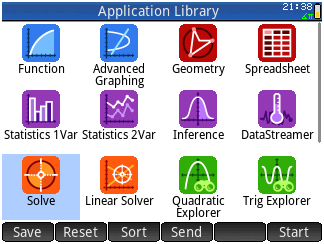
\includegraphics{Cap-FluxCarregues-HPP1.png}

    \item A continuació entrem les dues equacions que volem resoldre, utilitzant la variable \funsfbs{V} per a $|\cmplx{v}_2|$ i la variable \funsfbs{D} per a $\delta_2$.

        Al camp \funsfbs{E1} entrem l'equació: \funsfbs{-0.8-V*(1.05*(-2.8*COS(-D)-9.6*SIN(-D))+2.8*V)}, i al camp \funsfbs{E2} entrem l'equació: \funsfbs{-0.6+V*(1.05*(-2.8*SIN(-D)+9.6*COS(-D))-9.55*V)}.

        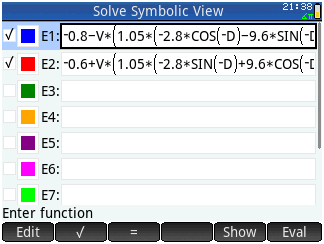
\includegraphics{Cap-FluxCarregues-HPP2.png}

    \item Tot seguit premem la tecla 
\includegraphics{HPPrime-Num.pdf} i entrem els valors inicials de les variables. Al camp \funsfbs{V} entrem: \funsfbs{1.05}, i al camp \funsfbs{D} entrem: \funsfbs{0}.

        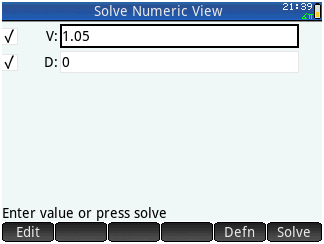
\includegraphics{Cap-FluxCarregues-HPP3.png}

    \item  Finalment premem el botó \hpbutton{Solve} i la calculadora ens dona  la solució.

        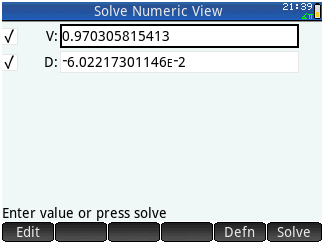
\includegraphics{Cap-FluxCarregues-HPP4.png}

\end{dingautolist}
